\section{Gestion de project}

\subsection{Planning prévionnel}

J'ai tout d'abort créer un diagramme de Gantt (voir annexe \ref{appendix:gantt}) pour m'aider à plannifer les différentes tâches que j'ai à faire. Pour élaborer ce diagramme de Gantt je me suis inspirer de la notion de \textit{sprints} de la méthode Agile Scrum \cite{scrum}. Un sprint, tel qu'utilisé dans ma gestion de projet, est une phase de developpement de l'application d'une durée de 1 semaine. Au terme d'un sprint, les fonctionnalités développer dans la semaines doivent être terminées, testées et prêtent à être disponible en production.

\begin{figure}
  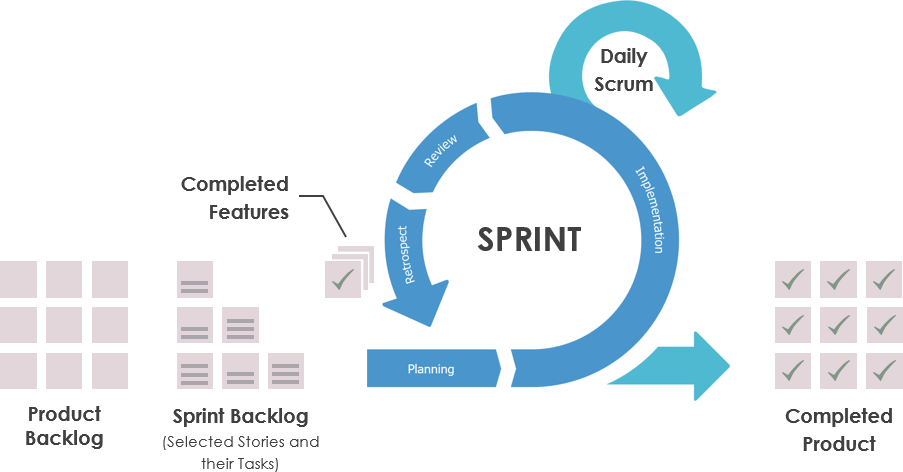
\includegraphics[width=.7\linewidth]{content/imgs/scrum_sprint.png}
  \caption{Sprint Scrum}
\end{figure}

Sur les 12 semaines semaines de stage, 7 semaines ont été consacré au developement de l'application. J'ai donc, en début de projet, défnis les fonctionnalités de  chacun des 7 sprints prévu. Les première semaines ont été consacré à la prise en main du sujet, aux recherches, à l'élaboration du cahier des charges et à la conception de l'architecture de l'application. Les dernières semaines ont été reservé au packaging final de l'application, au deploiement de l'application sur le \textit{Play Store} et à ce rapport.

Le planning du projet final, après modification de celui-ci au cours du projet, est disponible dans la partie \nameref{chapter:bilan} de ce rapport.

\subsection{Gestion de version (git)}

J'ai choisis d'utiliser le système de gestion de version Git avec le service d'hébergement Github pour héberger le projet afin de donner un accès rapide et complet à mon travail à mon enseignant référent et à ma superviseure de stage.

Github m'a aussi permis de créer des point de sauvergarde du projet, appelé \textit{release}, permettant de télécharger le code source des versions majeures de l'application avec commentaires de ce qui à changé depuis la dernière version ainsi que le fichier d'installation de l'application pour les appareils Android. La capture d'écran de la \textit{release} finale du projet est disponible dans l'annexe \ref{appendix:release}.











% eof
